92. \begin{figure}[ht!]
\center{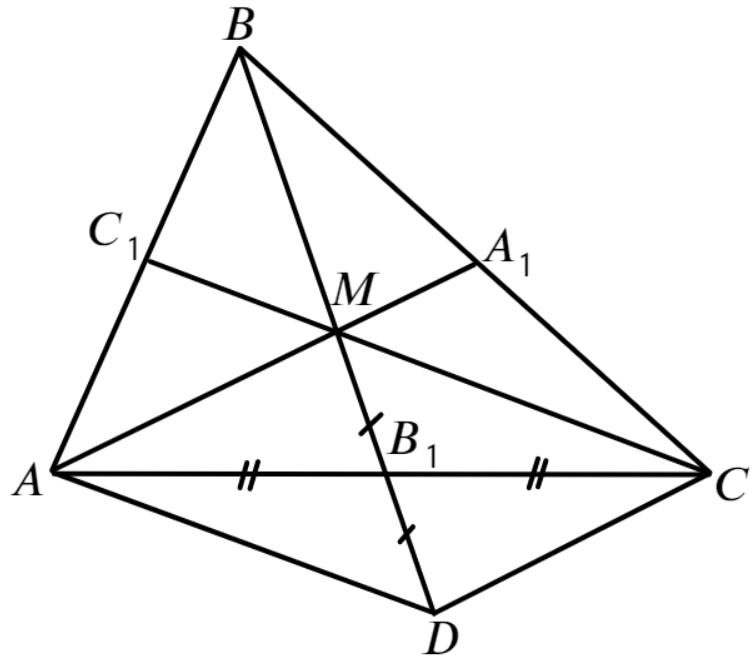
\includegraphics[scale=0.35]{g9-92.png}}
\end{figure}\\
Продолжим $MB_1$ так, чтобы $MB_1=B_1D.$ Тогда в четырёхугольнике $AMCD$ диагонали делятся точкой пересечения пополам, а значит он является параллелограммом и $CD=AM.$ Так как медианы делятся точкой пересечения $M$ в отношении $2:1,$ считая от вершины, стороны треугольника $CMD$ равны $2,\ \cfrac{8}{3}$ и $\cfrac{10}{3}.$ Так как $2^2+\left(\cfrac{8}{3}
ight)^2=\left(\cfrac{10}{3}
ight)^2,$ этот треугольник является прямоугольным и  $S_{\Delta CMD}=\cfrac{2\cdot\cfrac{8}{3}}{2}=\cfrac{8}{3},\ S_{AMCD}=2S_{\Delta CMD}=\cfrac{16}{3},\ S_{\Delta AMC}=\cfrac{1}{2}S_{ABCD}=\cfrac{8}{3}.$ Так как медианы делят любой треугольник на 6 равновеликих, $S_{\Delta ABC}=3S_{\Delta AMC}=8.$\\
